\documentclass{scrreprt}

\usepackage{aligned-overset}
\usepackage{amsmath}
\usepackage{amssymb}
\usepackage{bm}
\usepackage{chngcntr}
\usepackage[shortlabels]{enumitem}
\usepackage{hyperref}
\usepackage[utf8]{inputenc}
\usepackage{mathtools}
\usepackage{physics}
\usepackage{tabularx}
\usepackage{titling}
\usepackage{fancyhdr}
\usepackage{xfrac}
\usepackage[table]{xcolor}
\usepackage{pgfplots}

%% See https://tex.stackexchange.com/a/44954
\newcounter{myequation}
\makeatletter
\@addtoreset{equation}{myequation}
\makeatother

%% Fix equation numbering for scrreprt class.
\counterwithout{equation}{chapter}

\pgfplotsset{compat = newest}
\usepgfplotslibrary{patchplots}
\usetikzlibrary{intersections}
\usetikzlibrary{shapes}
\usetikzlibrary{shapes.geometric}
\usetikzlibrary{patterns}
\usepgfplotslibrary{fillbetween}

\author{Karsten Lehmann}
\date{SoSe 2021}
\title{Übung 13 Analysis - Weiterführende Konzepte}

\pagestyle{fancy}
\fancyhf{}
\lhead{\thetitle}
\rhead{\theauthor}
\lfoot{\thedate}
\rfoot{Seite \thepage}

\newcommand\skalprod[1]{\left\langle #1 \right\rangle}
\newcommand\nnorm[1]{\left\lvert\left\lvert\left\lvert #1 \right\rvert\right\rvert\right\rvert}

\begin{document}
\setcounter{chapter}{1}
\section*{Variation von Kurven}
\paragraph{Aufgabe 1:} (Graph einer Funktion als Kurve).
Gegeben sei eine stetige Funktion $f \colon [a, b] \to \mathbb{R}^N$.
Weiter sei $\gamma \colon [a, b] \to \mathbb{R}^{N + 1}$ definiert durch
\begin{flalign*}
  \gamma(t) &\coloneqq \qty\big(t, f(t)) &
\end{flalign*}
\begin{enumerate}[(i)]
\item Zeigen Sie, dass $\gamma$ eine Kurve ist.
  \subparagraph{Lösung:} Es ist zu zeigen, dass $\gamma$ stetig ist.

  Da $f$ stetig ist, ist auch die Abbildung
  $t \mapsto \qty\big(t, f(t)) = \gamma(t)$ stetig
  $\Rightarrow \gamma$ ist eine Kurve.

\item Beweisen Sie: Ist $\gamma$ stetig differenzierbar, so ist
  $\gamma$ von endlicher Variation.

  \subparagraph{Lösung:} $f$ ist stetig differenzierbar
  $\Rightarrow \underset{\makebox[0pt]{$L(\gamma)$ Länge der Kurve $\gamma$}}{
    \underbrace{\text{Var}_{[a, b]} \gamma}
  } < \infty$.

  $\gamma$ ist stetig differenzierbar, falls jede der Komponenten
  $x(t) = t, y(t) = f(t)$ stetig differenzierbar ist.
  Da $f$ stetig differenzierbar ist, trifft das auch auf $\gamma$
  zu.
  Aus Proposition 7.7.2 b) der Vorlesung -
  \textit{``Falls $\gamma$ stetig differenzierbar ist, dann ist
    $\text{Var}_{[a,b]}(\gamma) = \int_a^b \ldots$
  ''} folgt $\text{Var}_{[a,b]}(\gamma) < \infty$.

\item Berechnen Sie die Länge von $\gamma$ im Fall
  $f \colon [0, 1] \to \mathbb{R}, f(x) = \alpha x + \beta$

  \subparagraph{Lösung:}
  \begin{center}
    \begin{tikzpicture}
      \begin{axis}[
          axis lines=middle,
          xlabel=$x$,
          xmax = 1.3,
          xmin = -0.3,
          ylabel=$y$,
          ymax = 1.3,
          ymin = -0.3,
          yticklabels={,,},
        ]
        \addplot[
          domain = 0:1,
          very thick,
          blue,
        ] {0.8 * x + 0.2};
        \node[circle, fill, inner sep=2pt] at (0,0.2){};
        \node[circle, fill, inner sep=2pt] at (1,1){};
        \node at (-0.1, 0.2) {$\beta$};
        \node at (-0.15, 1) {$\alpha + \beta$};
      \end{axis}
    \end{tikzpicture}
  \end{center}
  Es gilt $\gamma(t) = \begin{pmatrix}
    t \\
    \alpha t + \beta
  \end{pmatrix} \Rightarrow \gamma'(t) = \begin{pmatrix}
    1 \\
    \alpha
  \end{pmatrix}$
  \[
    \Rightarrow \text{Var}_{[0, 1]}\gamma = \int_0^2\norm{\gamma'(t)}_2\,dt
    = \int_0^1\sqrt{1 + \alpha^2}\,dt = \sqrt{1 + a^2}
    = \norm{\qty\big(1, \alpha + \beta) - \qty(0, \beta)}_2
  \]

\end{enumerate}
\newpage
\paragraph{Aufgabe 2:} Untersuchen Sie, ob die Kurve
$\gamma \colon [0, 1] \to \mathbb{R}^2$ mit
\[
  \gamma(t) \coloneqq \begin{cases}
    \qty(t, t\cos\frac{\pi}{t}) & \text{für } t \in (0, 1] \\
    \qty\big(0, 0) & \text{für } t = 0
  \end{cases}
\]
von endlicher Variation ist.

\subparagraph{Lösung:} Wir setzen $\gamma(t) \coloneqq \begin{cases}
  t\cos\frac{\pi}{t} & \text{für } t \in (0, 1] \\
  0 & \text{für } t = 0
\end{cases}$ und $\gamma = \begin{pmatrix}
  t \\
  f(t)
\end{pmatrix}$.

Die Funktion $f$ ist auf $(0, 1]$ als Komposition stetiger Funktionen stetig.
Im Fall $t = 0$ gilt
$\abs{f(t) - f(0)} = \abs{t\cos\frac{\pi}{t}} \leq \abs{t - 0} \leq \epsilon
\eqqcolon \delta$. $\Rightarrow f$ ist in $0$ stetig.

Zerlegungungen $\Pi_n = \qty{
  t_0 = 1, t_1 = \frac{1}{n - 1}, t_2 = \frac{1}{n - 2}, \ldots,
  t_n = \frac{1}{n - (n - 1)} = 1
}$
\[
  \Rightarrow \gamma\qty\big(t_k) = \begin{pmatrix}
    x_k \\
    y_k
  \end{pmatrix} = \frac{1}{n - k} \cdot \begin{pmatrix}
    1 \\
    \cos\qty\big((n - k) \pi)
  \end{pmatrix} = \frac{1}{n - k} \cdot \begin{pmatrix}
    1 \\
    (-1)^{n - k}
  \end{pmatrix}
\]
Durch Verbindung der Punkte $\gamma(t_0), \gamma(t_1), \ldots, \gamma(t_n)$
entsteht ein Streckenzug.
Es gilt
\begin{flalign*}
  \text{Var}_{[0, 1]} \qty(\gamma, \Pi_n)
  &= \sum_{k = 1}^n \norm{\gamma\qty(t_k) - \gamma\qty(t_{x - 1})}_2
  = \sum_{k = 1}^n \qty\Big(\qty\big(x_k - x_{x - 1})^2 + \qty\big(y_k - y_{k - 1})^2)^{\frac{1}{2}} & \\
  &\geq \sum_{k = 1}^n \abs{y_k - y_{k - 1}} \\
  &\geq \sum_{k = 2}^n \qty(\frac{1}{n - k} + \frac{1}{n - k + 1}) \\
  &\geq \sum_{k = 2}^{n - 1} \frac{1}{n - k} \overset{j = n - k}=
  \sum_{j = 1}^{n - 2} \frac{1}{j} \overset{n \to \infty}\longrightarrow \infty
\end{flalign*}
$\Rightarrow \text{Var}_{[a, b]} \gamma = \infty$

\paragraph{Aufgabe 3:}
\begin{enumerate}[(i)]
\item Skizzieren Sie die Kardioide $\gamma \colon [0, 2\pi] \to \mathbb{R}^2$
  definiert durch
  \[
    \gamma(t) \coloneqq \qty\Big(\qty\big(1 - \cos t)\cos t, \qty\big(1 - \cos t) \sin t)
  \]
  und berechnen Sie deren Länge $L = \text{Var}_{[0, 2\pi]}(\gamma)$

  \subparagraph{Lösung:} $\gamma(t) = r(t) \cdot \begin{pmatrix}
    \cos t \\
    \sin t
  \end{pmatrix}, r(t) = 1 - \cos t, r(t) \leq 0, t \in [0, 2\pi]$
  und $r'(t) = \sin t$.
  \newpage
  \begin{center}
    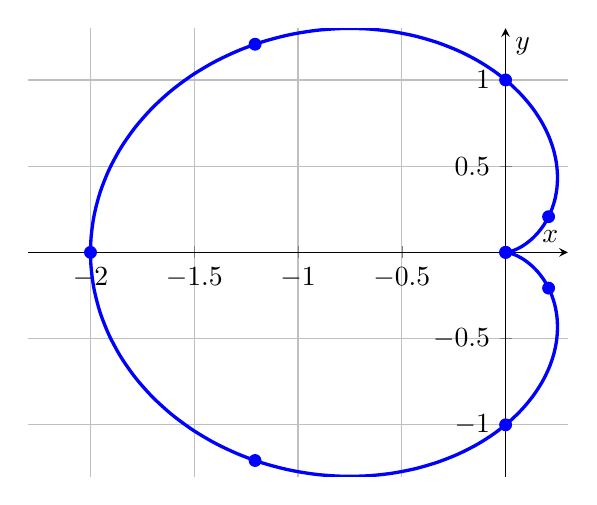
\begin{tikzpicture}
      \begin{axis}[
          axis lines=middle,
          grid = both,
          xlabel=$x$,
          xmax = 0.3,
          xmin = -2.3,
          ylabel=$y$,
          ymax = 1.3,
          ymin = -1.3,
        ]
        \addplot[
          data cs = polar,
          domain = 0:360,
          very thick,
          blue,
          smooth,
          samples = 90,
          ] ({x}, {1 - cos(x)});
          \pgfplotsforeachungrouped \k in {0,...,8}{
            \pgfmathsetmacro\x{\k * 360 / 8}
            \pgfmathsetmacro\y{1 - cos(\x)}
            \edef\temp{\noexpand\node[
                circle,
                draw,
                fill,
                inner sep=1.5pt,
                blue,
              ] at ({\x}:\y) {};}
            \temp
        }
      \end{axis}
    \end{tikzpicture}
  \end{center}
  Graph der Kurve $\gamma$. Dabei sind die Punkte
  $\gamma\qty(\frac{k\pi}{4})$ für $k = 0, \ldots, 8$ markiert.

  $\gamma$ ist stetig differenzierbar mit
  \begin{flalign*}
    \gamma'(t) &= \begin{pmatrix}
      x'(t) \\
      y'(t)
    \end{pmatrix} = r'(t) \cdot \begin{pmatrix}
      \cos t \\
      \sin t
    \end{pmatrix} + r(t) \cdot \begin{pmatrix}
      -\sin t \\
      \cos t
    \end{pmatrix} & \\
    &= \begin{pmatrix}
      \sin t \cdot \cos t + (1 - \cos t)(- \sin t) \\
      \sin^2 t + (1 - \cos t)\cos t
    \end{pmatrix}
    = \begin{pmatrix}
      - \sin t + 2 \sin t \cdot \cos t \\
      \cos t - (\cos^2 t - \sin^2 t)
    \end{pmatrix} \\
    &= \begin{pmatrix}
      - \sin t + \sin(2t) \\
      \cos t - \cos(2t)
    \end{pmatrix} \\
    \Rightarrow \norm{\gamma'(t)}_2^2 &= \qty\Big(-\sin t + \sin(2t))^2
    +\qty\Big(\cos t - \cos(2t))^2 \\
    &= \sin^2 t - 2 \sin t \sin(2t) + \sin^2(2t) + \cos^2 t - 2 \cos t \cos(2t) + \cos^2(2t) \\
    &= 2 \qty\Big(1 - \qty\big(2 \sin^2 t \cos t + \cos t \underset{1 - 2 \sin^2 t}{\underbrace{(\cos^2 t - \sin^2t)}})) \\
    &= 2 \qty\big(1 - \underset{\cos\qty(\frac{t}{2} + \frac{t}{2})}{\underset{\uparrow}{\cos t}})
    = 2 \qty\Big(1 - \qty(1 - 2\sin^2 \frac{t}{2})) \\
    &= 4 \sin^2 \frac{t}{2} \\
    \Rightarrow \text{Var}_{[0, 2\pi]}(\gamma) &= \int_0^{2\pi} \norm{\gamma'(t)}_2 \,dt
    = 2 \int_0^{2\pi} \abs\Big{\underset{\geq 0}{\underbrace{\sin \frac{t}{2}}}}\,dt
    = 0 \int_0^{2\pi} \sin \frac{t}{2}\,dt \\
    &= 2 \qty[\cos \qty(\cos\frac{t}{2})(-1) 2]_0^{2\pi} = -4 \qty\big(\cos \pi - \cos 0) \\
    &= 8
  \end{flalign*}
\end{enumerate}

\end{document}